\documentclass[10pt]{article}
\usepackage{NotesTeX}
\usepackage{graphicx}
%\usepackage{sidenotes}
%\usepackage{lipsum}

\title{{\Huge Summary}\\{\Large{DianNao: A Small-Footprint
High-Throughput Accelerator for Ubiquitous Machine-Learning
\footnote{Tianshi Chen. DianNao: A Small-Footprint
High-Throughput Accelerator for Ubiquitous Machine-Learning.
ASPLOS, 2014.}}}}
\author{Cui Weihao}    
\affiliation{SJTU}
\emailAdd{reallygoodhao@126.com}
\begin{document}
    \maketitle
    \flushbottom
    \newpage
    \pagestyle{fancynotes}
    \part{Brief Introduction}
    In this paper, a novel machine-learning accelerator is designed for
    large-scale CNNs and DNNs, with a special emphasis on the impact
    of memory on accelerator design, performance and energy.
    \section{Main Contributions}
    \begin{itemize}
        \item A synthesized (place \& route) accelerator design for
        large-scale CNNs and DNNs, the state-of-the-art
        machine-learning algorithms.
        \item The accelerator achieves high throughput in a small area,
        power and energy footprint.
        \item The accelerator design focuses on memory behavior, and
        measurements are not cicumscribed to computational tasks, they
        factor in the performance and energy impact of memory transfer.
    \end{itemize}
    \section{Composition of Accelerator}

    As shown on the right:
    \begin{marginfigure}
        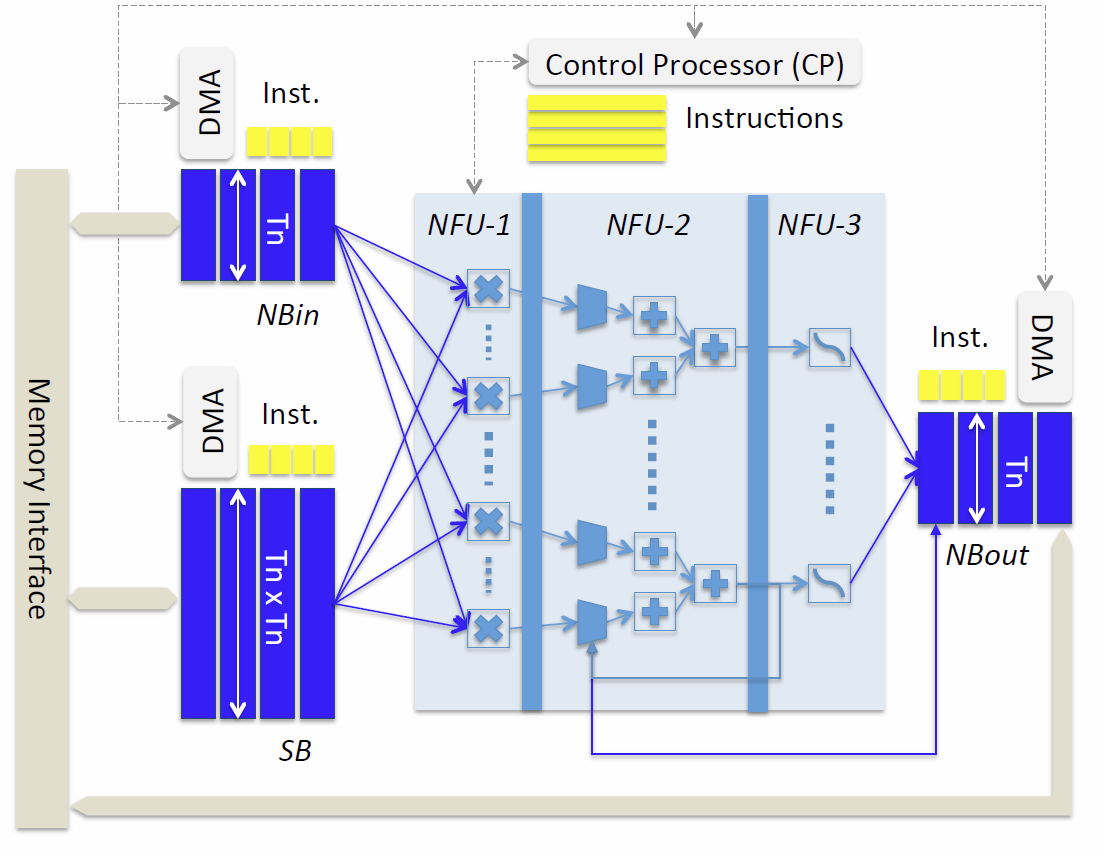
\includegraphics[width=\marginparwidth]{composition.png}
    \end{marginfigure}
    \begin{itemize}
        \item Storage: an input buffer for input neurons (NBin), an out
        put buffer for output neurons (NBout), a third buffer for
        synaptic weights (SB).
        \item Computations: Neural Functional Unit.
        \item Control of Accelerator: Control Logic and  layer code.
    \end{itemize}
    %\section{Exprimental Results}
    %\flushbottom
    %\newpage
    %\pagestyle{fancynotes}
    \part{Details of the Accelerator's design}
    \section{Neural Functional Unit (NFU)}
    The spirit of the NFU is to reflect the decomposition of a layer,
    which is included in CNNs and DNNs, into computational blocks.
    \begin{itemize}
        \item Arithmetic operators

        The computations of each layer type can be decomposed in
        either 2 or 3 stages, e.g. , for classifer layers: 
        multiplication of synapses $\times$ inputs, additions of
        all multiplications, sigmoid. So are the convolutional
        layers, pooling layers and so on.
        \item Staggered pipline

        We can pipeline all 2 or 3 aforementioned operations in
        single layer, but the pipeline must be staggered: the third
        stage such as sigmoid is only active after all additions have 
        been performed. From now on, we refer to stage n of the NFU
        pipeline as NFU-n.
        \item NFU-3 function implementation

        As proposed in the literature \sn{D. Larkin, A. Kinane, 
        V. Muresan, and N. E. O'Connor. An Efficient Hardware
        Architecture for a Neural Network Activation Function
        Generator. In J. Wang, Z. Yi, J. M. Zurada, B.-L. Lu, and
        H. Yin, editors, ISNN (2), volume 3973 of Lecture Notes in
        Computer Science, pages 1319-1327. Springer, 2006.}
        the sigmoid of NFU-3 can be efficiently implemented using
        piecewise line iterpolation($f(x) = a_i \times x + b_i, x
        \in [x_i, x_i + 1 ]$) with negligible loss of accuracy.
        The segments used in the implementation are stored in a
        small RAM which allows to implement any function, not just
        a sigmoid (e.g., hyperbolic tangent, linear functions, etc
        )
        \item 16-bit fixed-point arithmetic operators

        In the paper, it uses 16-bit fixed-point arithmetic
        operators instead of word-size (e.g., 32-bit)floating-point
        operators. While it may seem surprising, there is ample
        evidence in the literature that even smaller operators
        (e.g., 8bits or even less) have almost no impact on the 
        accuracy of neural networks as shown in the right image.
        \begin{marginfigure}
            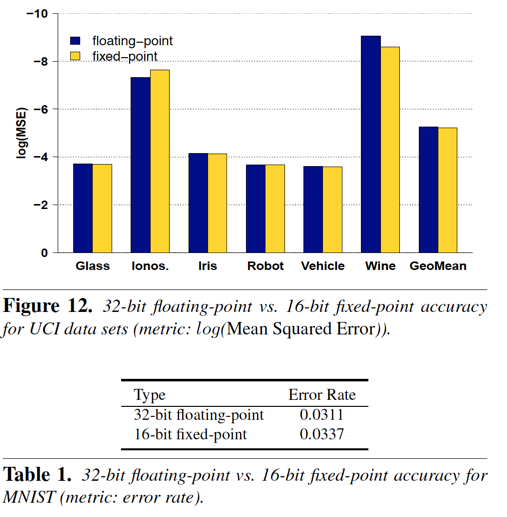
\includegraphics[width=\marginparwidth]{arithmetic.png}
        \end{marginfigure}

        Using a 16-bit fixed-point arithmetic saves the area and
        power than the 32-bit floating-point operators.
    \end{itemize}
    \section{Storage: NBin, NBout and SB}
    A scratchpad in a dedicated accelerator realized the best of
    both words: efficient storage, and both efficient and easy
    exploitation of locality because only a few algorithms have to be
    manually adapted.

    How the storage part of the accelerator is organized and which
    limitations of cache architectures it overcomes will be explained
    below.
    \begin{itemize}
        \item Split buffers
        
        The storage of the accelerator have been split into three 
        structures: an input buffer(NBin), an output buffer(NBout) and
        a synapse buffer (SB).
        Here are the benefit of the spliting:
        \begin{enumerate}
            \item \textbf{\emph{Width}} 
            It can tailor the SRAMs to the appropriate read/write
            width. Splitting storage into dedicated structures allows
            to achieve the best time and energy for each read request.
            \item \textbf{\emph{Conflicts}}
            It can avoid conflicts, as would occur in a cache. It is
            especially important for keeping the size of the storage
            structures small for cost and energe (leakage) reasons.
            Split storage and precise knowledge of locality behavior
            allows to entirely remove data conflicts.
        \end{enumerate}
        \item Exploiting the locality of inputs and synapses
        \begin{enumerate}
            \item \textbf{\emph{DMAs}}
            For spatial locality, three DMAs, one for each buffer(two
            load DMAs, one store DMA for outputs) are implemented.
            \item \textbf{\emph{Rotating NBin buffer for temporal reuse of
            input neurons}}
            The neural networks have many layers. The inputs of all
            these layers are split into chunks which fit in NBin, and 
            they are reused by implement NBin as a \emph{circular 
            buffer}, which is implemented by software. 
            \item \textbf{\emph{Local transpose in NBin for pooling layers}}
            There is a tension between convolutional and pooling layers for
            the data structure organization of (input) neurons. The tension
            is resolved by interleaving the data in NBin as it is loaded.
        \end{enumerate}
        \item Exploiting the locality of outputs

        Since the partial output sum of the neurons is computed for a later
        chunk of input neurons contained in NBin, two issues occurs.
        \begin{enumerate}
            \item \textbf{\emph{Dedicated registers}}
            It is inefficient to let the partial sum exit the NFU pipline 
            and then re-load it into the pipeline for each entry of the NBin 
            buffer. So dedicated registers are introduced in NFU-2 to store
            partial sums.
            \item \textbf{\emph{Circular buffer}}
            For reusing the data in NBin and rotating them, NBout is not
            only connected to NFU-3 and memory, but also to NFU-2: one entry
            of NBout can be loaded into the dedicated registers of NFU-2, and
            these registers can be stored in NBout. 
        \end{enumerate}
    \end{itemize}
    \section{Control and code}
    \begin{itemize}
        \item Control processor(CP)

        For now this accelerator use \emph{control instructions}.A layer
        execution is broken down into a set of instructions, which are stored
        in an SRAM associated with the CP. Every instructions has five slots,
        corresponding to the CP itself, the three buffers and NFU. The CP 
        drives the execution of the DMAs of the three buffers and the NFU.
        \item Layer Code

        Because of the CP instructions, there is a need for code generation.
        Three dedicated code generators are implemeted for the three layers.
    \end{itemize}
    %\flushbottom
    %\newpage
    %\pagestyle{fancynotes}
    \part{Summary}

    This paper show it is possible to design a machine-learning accelerator 
    capble of both high performance in a very small area footprint and energy
    reduction.
\end{document}